\chapter{Testrig}
\section{Introduction}
When designing a complex system such as a hybrid vehicle, continuously being
able to test the system is important to validate that the requirements are met
and to verify the models. To be able to do a full system test, the car has to be
physically run on a track. This can be cumbersome, or in the case of the London
track, impossible at times. Therefore, a test rig is designed and built. The
design process uses the V-model approach with a set of live requirements and
continuous unit and integration testing. The overall goal is to not only be able to do a faithful simulation of the SEM-track in London, but to be able to supply any track (with certain limitations on power and speed demands) to the test rig.

\section{Requirements}
The requirements on the test rig are designed to capture the essential demands
on the system. Firstly, the high level User requirements are set. These are set
to capture the problem and to describe the goal of designing the
system~\cite{ibm_req}. The User requirements are then developed into the System
requirements that describe the limitations and demands on the system and its
subsystems.

\section{Design decisions}
During the design of the testrig the team faced a few issues with multiple possible solutions. The most impactful and important decisions are briefly explained here.

\subsection{Concept design}\label{sec:testrig_design_concept}
Two basic concepts for the testrig were incepted. The first concept was to remove the driving wheel and attach a motor that was to apply the proper torque at all times to simulate the forces that would act on Elba in the real world.

The second concept was to construct two rollers that Elba would stand on with its driving wheel and apply a torque to one of the rollers via a DC motor.

The team decided to continue working with the roller concept. Reasons for this are explained further in \ref{sec:discussion_testrig_concept}.

\subsection{Regeneration}
Another problem that needed a solution was the handling of regenerated current. As seen in Figure \ref{fig:testrig_negative_forces} the forces produced by the testrig will at almost all points of the track be opposite to Elbas travelling direction. This means that the DC motor will work as a generator most of the time, since the torque and speed will be in opposite directions. Many different ideas of ways to solve this problem were tossed around, but all with the fundamental idea to have power resistors connected where excess energy could be dissipated. One idea was to manually switch to dissipating energy when needed. The final solution included a supercapacitor to store energy temporarily to be used when simulating a downhill, and a way of automatically burning excess when the supercapacitor was fully charged. The complete setup is explained with greater detail in \ref{sec:testrig_hardware}.

\subsection{Control}\label{sec:testrig_design_control}
The desired output of the testrig is the combined external forces that affect the car at any given time on a track. This means that the output to control is the torque on the rollers. The team chose between two ways of doing this. The first was to measure the torque directly using an appropriate sensor. The second idea was to measure the current applied to the motor and calculate the torque from the current. 

The team decided to use current control. Further explanation as to why this was chosen can be seen in \ref{sec:discussion_testrig_control}.

\section{Hardware}\label{sec:testrig_hardware}
The testrig is composed of two rollers mounted on a metal frame together with a
DC motor and an encoder to keep track of the speed
of the motor. The motor is connected to the rollers by sprockets and chain with
a gearing ratio of two. A model of the system can be seen in Figure \ref{fig:testrig_hardware}.

\begin{figure}[H]
    \centering
    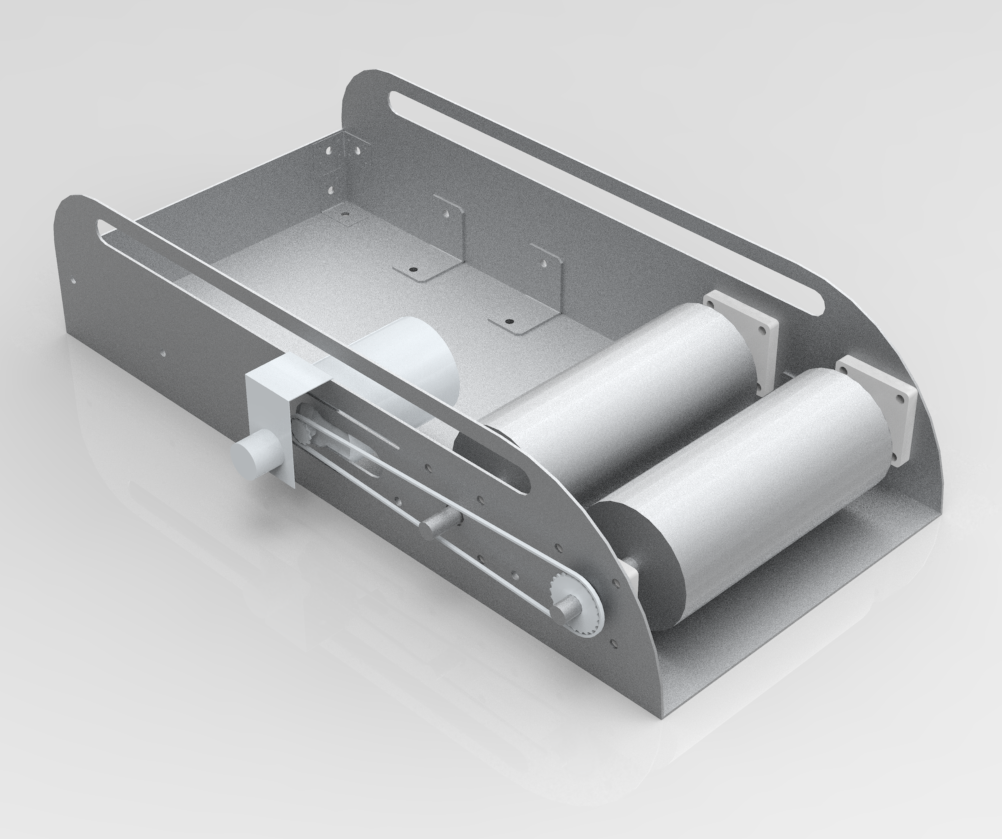
\includegraphics[width=0.75\textwidth]{./img/testrig_hardware.png}
    \caption{CAD model of the testrig without the chainguard for increased visibility.}
    \label{fig:testrig_hardware}
\end{figure}

To control the DC motor an Arduino Mega 2560 microcontroller
calculates what current should be applied to the motor (explained further in section \ref{sec:cardynamics} and \ref{sec:rigdynamics}), this reference signal
is used by a ESCON driver to control the current in a local feedback loop.

The current generated by the DC motor is stored in a supercapacitor, connected in parallell to motor driver. The microcontroller monitors this voltage via a voltage divider since the input voltage to an Arduino Mega 2560 can be max 5 V. If more energy is generated than the supercapacitor can handle, the microcontroller will close a relay between six parallel power resistors and ground, and it will remain closed until the supercapacitor has discharged to a lower limit when the microcontroller will open the relay and make the supercapacitor able to recharge again.

A problem that exists with the Arduino microcontroller is that it is exposed to disturbances from the motors and ICE. These disturbances has at times made the microcontroller to crash and restart, which of course affects its abilities to control the energy dissipation from the supercapacitor. To ensure that the supercapacitor does not exceed the maximum rated voltage of 48 volt the voltage is monitored by a person with an externally applied voltmeter. If the voltage rises above 48 volt due to a crashed microcontroller an emergency stop button is pressed which inhibits the testrig motor driver from generating more energy. 

The upper level when the microcontroller should close the relay was decided by the specifications of supercapacitor, since it should not be charged beyond 48 V. To have some margin of error the upper limit was set to 47 V. The lower limit of the voltage should not be too low since the motor will have different dynamics depending on voltage applied. Also it shouldn't be too close to the upper limit in order to avoid the relay to constantly be turned on and off. It was decided to set the lower limit to 45 V. The system is connected to a 45 V voltage supply via a rectifier to avoid generated current to flow into the power supply.

A basic schematic of the setup can be seen in
Figure~\ref{fig:testrig_schematic}.

\begin{figure}[H]
    \centering
    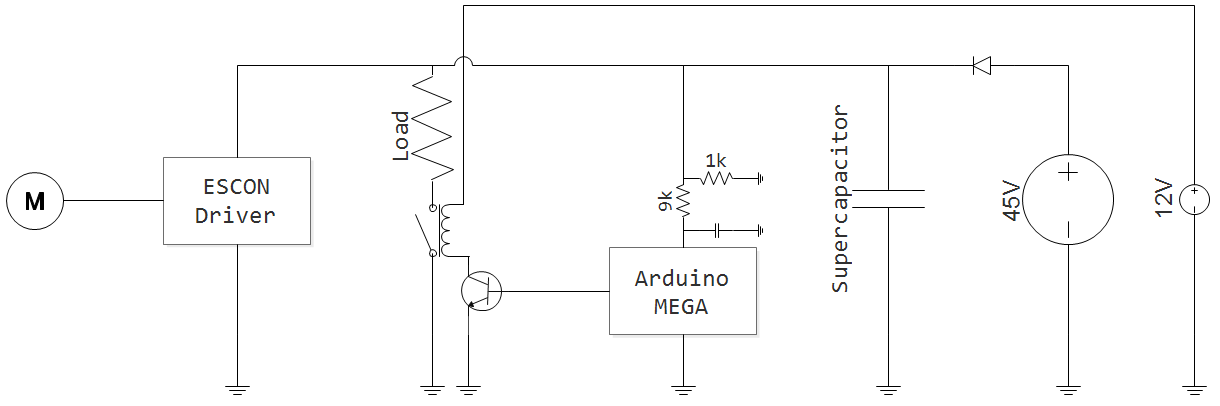
\includegraphics[width=\textwidth]{./img/testrig_schematic.png}
    \caption{Schematic of testrig wiring to control the voltage supplied to the driver.}\label{fig:testrig_schematic}
\end{figure}

\section{Car dynamics}\label{sec:cardynamics}
The calculations in this section are in many ways the same as the calculations
given in the previous teams report in Appendix~\ref{app:elba2015}. Though some
of the equations are repetition of what was done last year, they are
done here again with some improvements and more references to make the
derivations of the equations clearer.

When simulating a track, one needs to know the force exerted by the environment
on the car. A graphical representation of the forces that act on the car is
given in Figure~\ref{fig:testrig_elbadynamics}.
\begin{figure}[H]
    \centering
    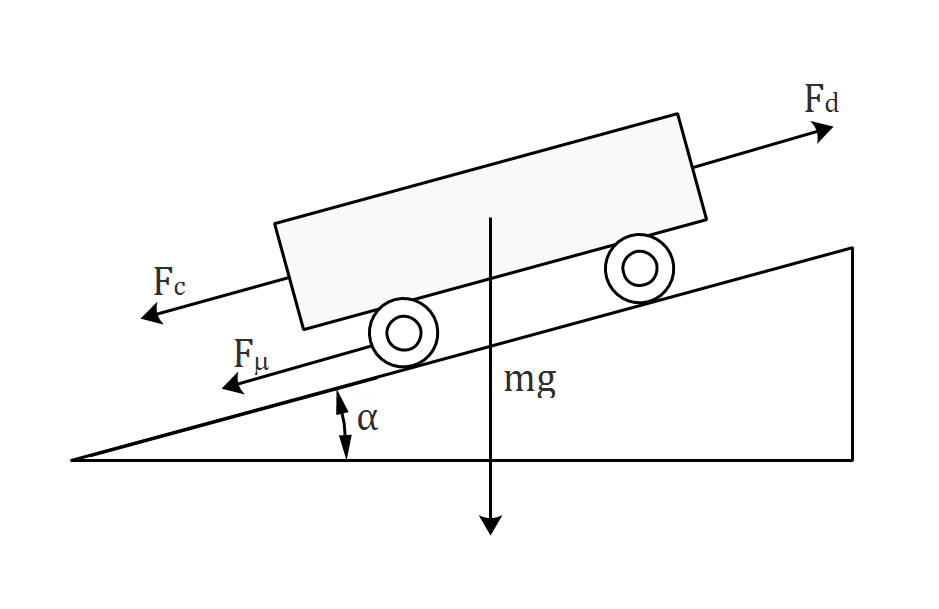
\includegraphics[width=0.5\textwidth]{./img/testrig_elbaforces.png}
    \caption{Dynamic model of Elba.}\label{fig:testrig_elbadynamics}
\end{figure}
The motion equations on the system are 
\begin{equation} \label{eq:testrig_cardynamics}
    m\ddot{x} = F_d - mg\sin{\alpha} - F_c - F_{\mu},
\end{equation}
where $F_d$ is the effective driving force of the car, $m$ is the mass of the
car and $alpha$ is the slope from the horizontal plane. The resistance terms
$F_c$ and $F_{\mu}$ are air and road resistance, respectively. The air drag $D$
around an object can be calculated as~\cite{nakayama2002}
\begin{equation} \label{eq:testrig_airdrag}
    D = C_D A \frac{\rho v^2} {2}
\end{equation}
with object velocity $v$, surface area vertical to the movement direction $A$
and air density $\rho$. Most terms in Equation~(\ref{eq:testrig_cardynamics})
are constant throughout a driving instance. Rewriting to
\begin{equation} \label{eq:testrig_csimple}
    C_{tot} = \frac{C_D A \rho} {2}
\end{equation}
yields a simplified equation that only depends on the velocity,
\begin{equation} \label{eq:drag}
    F_D = C_{tot}v^2.
\end{equation}
The total drag coefficient $C_{tot}$ will depend on the vertical area, the density of
air and the drag coefficient $C_D$. The air density is considered to be constant
and is known. The area of Elba can be estimated using simple methods. Finally,
the air drag coefficient $C_D$ is unique to each and every object and is
determined experimentally. For this project, the estimations given for a
passenger car is used. Detailed calculations and values are given in
Appendix~\ref{app:rigdata}. 

% This section is under construction. Need some reference/experiment on how to 
% model rolling friction.
The rolling friction of a car is modeled as a step function, being non-zero at
all velocities that are not zero.

With the air drag, rolling friction and gravity terms known, only two terms of
Equation (\ref{eq:testrig_cardynamics}) are unknown. To fully model the cars
dynamics, the inertia term needs to be modeled. Since the weight of the vehicle
is known, $\ddot{x}$ needs to be derived for an accurate system model.
Knowing the radius of the rollers and the cars wheels, the linear acceleration
can be calculated by measuring the rotational acceleration on the roller. This
is done by an incremental encoder on the roller shaft. Rotational speed is
calculated in the microcontroller and rotational acceleration is derived from
rotational speed. Using the roller radius, $r_{r}$, the linear acceleration
is calculated.

Rewriting Equation~\ref{eq:testrig_cardynamics}, \ref{eq:drag} and the friction force gives the
desired linear testrig simulation force on the right hand side,
\begin{equation} \label{eq:simulationforce}
    F_{tr} = m\ddot{x} + mg\sin{\alpha} + C_{tot}\dot{x}^2 + F_{\mu}.
\end{equation}

Using the height profile of the London track and the plant model of Elba, $F_{tr}$ during an entire lap could be simulated, as shown in Figure (\ref{fig:testrig_negative_forces}).

\begin{figure}[H]
    \centering
    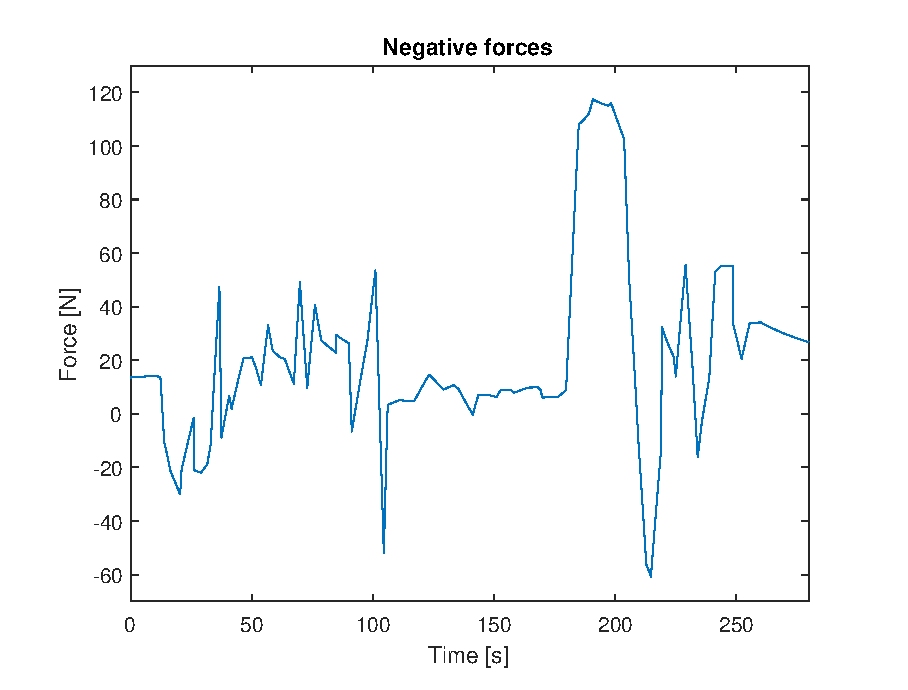
\includegraphics[width=\textwidth]{./img/testrig_negative_forces.eps}
    \caption{Negative forces acting upon Elba in one lap.}\label{fig:testrig_negative_forces}
\end{figure}

\section{Testrig dynamics}\label{sec:rigdynamics}
In order to let the testrig output the correct linear force to the car, the
controller for the testrig need to know the dynamics of the testrig itself. This
is to compensate for internal frictions and inertias. The driveline of the
testrig has two separate steps, the motor and the roller, connected by a chain
gear with gear ratio $n_{chain}$. A principle schematic of the testrig from
motor to roller is displayed in Figure~\ref{fig:testrig_testrigdynamics}.
\begin{figure}[H]
    \centering
    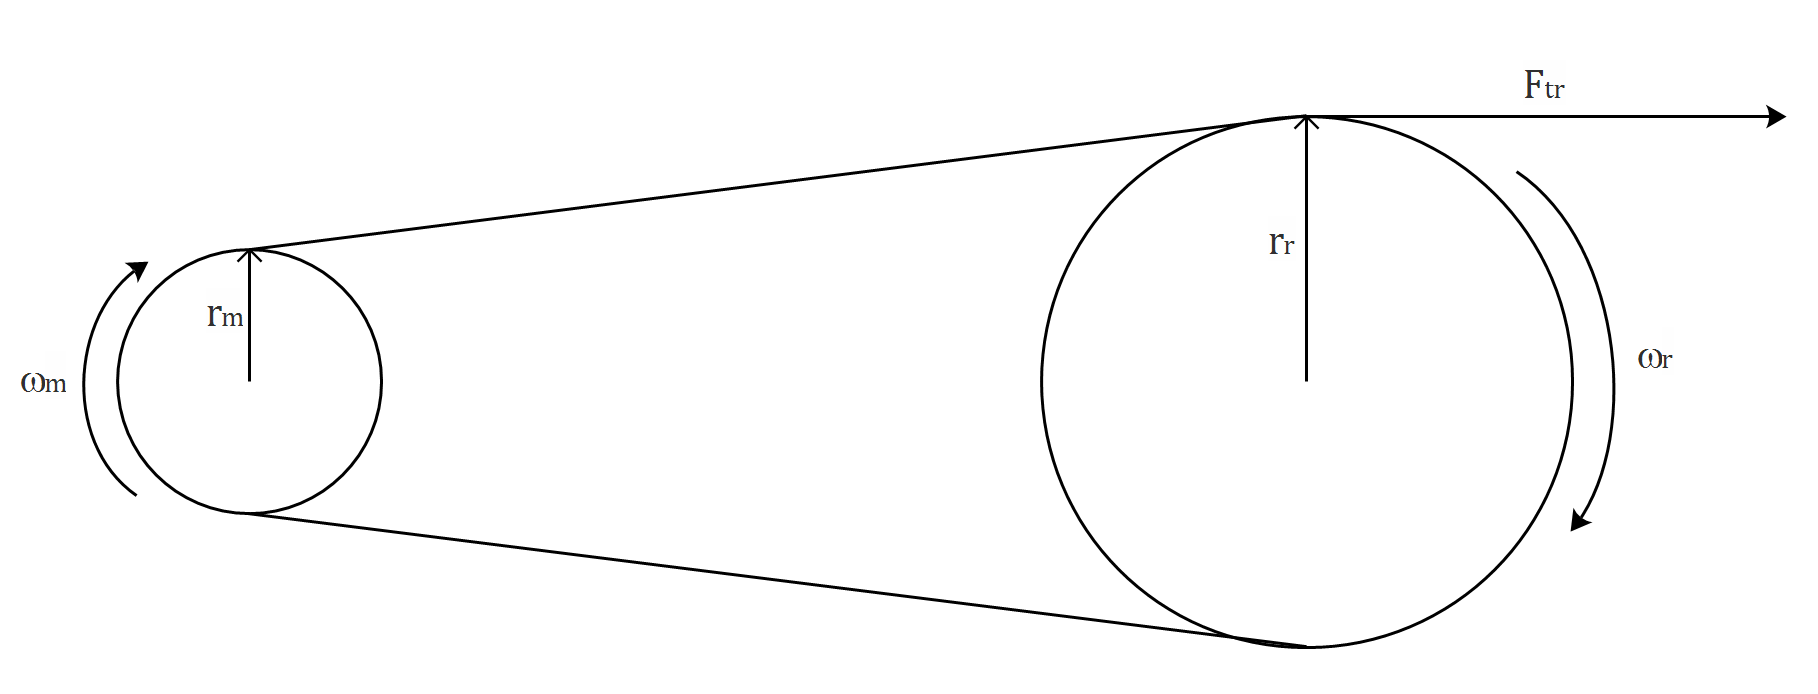
\includegraphics[width=0.9\textwidth]{./img/testrig_rollerschematic.png}
    \caption{Principle schematic of the testrig from motor to roller.}\label{fig:testrig_testrigdynamics}
\end{figure}
The dynamic equations for the rollers are
\begin{equation} \label{eq:testrig_rollerdynamics}
    J_r \dot{\omega}_r = F_{tr}r_r - d_r \omega_r - \mu_r,
\end{equation}
%Inte 100% säker på att Ftr blir rätt här /Emil

where $J_r$ is the inertia of the rollers and $\omega_r$ is the rotational velocity
of the roller. The frictional terms are the viscous friction $d_r$ and the
constant friction $\mu_r$ which is modelled by the Karnop model.

Connecting the rollers and the motor is a chain gear. It is modelled as a
generic gear box. The gearbox model has no internal friction. There is always friction in a
chain gear but it is expected that this friction will be incorporated in the
total system model and the friction free representation is deemed adequate.
Using Equation (\ref{eq:testrig_rollerdynamics}) and (motor model) along with
the gearbox model, the total testrig dynamic model becomes

\begin{equation} \label{eq:testrig_totaldynamics} 
    T_m = \frac{F_{tr} r_r + J_{tot} \dot{\omega}_m + d_{tot} \omega_m + \mu_{tot}}{n},
\end{equation}

%TODO: Kanske fel i ekvationen, möjligt korrekt:
%\begin{equation} \label{eq:testrig_totaldynamics2} 
%    T_m = \frac{F_{tr} r_w + J_{tot} \dot{\omega}_m + d_{tot} \omega_m + \mu_{tot}}{n_1 n_2},
%\end{equation}

with motor torque $T_m$, simulation force $F_{tr}$ and motor rotational velocity
$\omega_m$. The inertia term is the combined inertia of the motor and
roller,
\begin{equation} \label{eq:totalinertia}
    J_{tot} = J_m + J_r \frac{1} {n^2}.
\end{equation}
The friction terms are combined terms as well, namely
\begin{equation} \label{eq:testrig_totalvfric}
    d_{tot} = d_m + d_r \frac {1} {n}
\end{equation}
and
\begin{equation} \label{eq:testrig_totalfric}
    \mu_{tot} = \mu_m + \mu_r.
\end{equation}

The power $P_m$ required for the motor on the testrig was calculated as
\begin{equation} \label{eq:testrig_motorpower}
	P_m = T_m \omega_m
\end{equation}

Using the London track and the plant model of Elba, $P_m$ during one lap could be simulated, as shown in (\ref{fig:testrig_power_required}).

\begin{figure}[H]
    \centering
    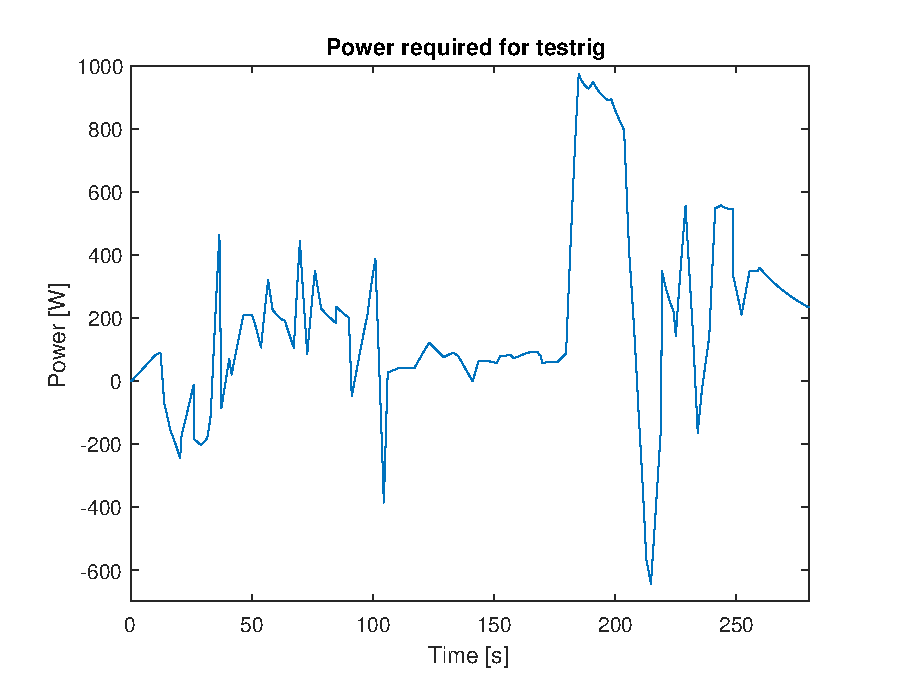
\includegraphics[width=\textwidth]{./img/testrig_power_required.eps}
    \caption{Power required for the motor on the testrig.}\label{fig:testrig_power_required}
\end{figure}

Figure (\ref{fig:testrig_power_required}) shows that the maximum required power from the testrig motor is 1 kW.

\section{Identification}
Having obtained the dynamic equations of the system in Equation
(\ref{eq:testrig_totaldynamics}), a system identification is done to determine
the parameters of the system. The parameters are then used in the open loop
current/torque controller. The controller is run in open loop for the
torque, i.e.\ there is no direct torque feedback. To get the desired torque
output, the current is controlled via a closed loop feedback controller and
torque is calculated from the actual current. With a knowledge about motor
parameters and the dynamics of the system, the actual torque can be estimated. 

\subsection{Motor parameters}
To acquire the motor parameters  calculations had to be made, since it did not exist any datasheet to the DC motor in use. The motor parameters needed was the internal resistance, $R_{a}$, and the motor constant, $k_{\phi}$. The motor was run at idle for two different voltage levels and the current and the speed in terms of revolutions per minute (RPM) where noted for those specific voltage levels. The speed in angle velocity was calculated from RPM, and together with the current for two different instances of voltage level, $R_{a}$ and $k_{\phi}$ was calculated. The equation
\begin{equation}
\label{eq:motor_parameters}
    U = R_a I + k_{\phi} \omega
\end{equation}
found in \cite{elektroteknik2013} was used in an equation system to derive the internal resistance and motor constant.

\subsection{Hardware setup}
The testing is processed in Matlab and Simulink. Input data is gathered from the
real system and is then fed into the model afterwards for model comparison. This
has the advantage of doing a physical test once, recording the data and the be
able to test it on the model without setting up the test system again. Output
data from the testrig, rotational velocity of the motor, is also collected and
used as a reference for the model.

To measure motor voltage, a computer oscilloscope was used (Digilent Analog
Discovery 2). The oscilloscope has an open C API, allowing its interface to be
customized. An S-Function block was made that allowed the oscilloscopes
measurements to be directly recorded in Simulink. To make sure that the model
ran in real-time in Simulinks normal mode, a Real-time constraint block was
added to the simulink model. The probes of the oscilloscope were attached to
the positive and negative pole of the motor. All data was recorded into a
Simulink Datastruct that could then be used as input for the model. 

For recording the output data, rotational velocity, an incremental quadrature
encoder was used. The encoder pulse data was recorded and converted into
velocity by the test rig ECU\@. The Simulink model for the ECU was run on external
mode and encoder data was saved. 

Because of software limitations, the oscilloscope and the testrig ECU can not be
run in the same Simulink instance. This means that two separate models are run
simultaneously, one recording the input and one recording the output.

\subsection{Identification process}
The testrig is a rather simple system in principle. It consists of an electric
motor attached to a load with inertia and friction, see
Figure~\ref{fig:testrig_dcmotor_model}.  This is consistent with most standard
models of an electric motor (see for example~\cite{beloiu2014},
\cite{reglerteknik2006} and~\cite{modeling1994}) and the systems dynamics are
therefore assumed to be well known mathematically. When the mathematical model
of a dynamic system is known, a parametrized model based on the real
physical parameters of the system can be used in the identification process.
This is known as a Gray-box model~\cite{modeling1994}. This approach is
beneficial because the unknown parameters are based upon real physical
parameters and are thus easier to estimate and relate to the model. 

The goal of the system identification is to estimate the unknown parameters of the
system well enough so that the testrig can be current controlled based on a 
desired net output torque. This requires knowledge about friction losses that
occur between the torque source and the torque output. Model accuracy is therefore
important but must be weighed against needed processing power in the microprocessor
used to control the rig. A higher-order model will require more processing power
to be solved online and might negatively affect the real-time performance of the
system. To find a balance between accuracy and processing power, an iterative
identification process is used, described in Figure 14.1 in~\cite{modeling1994}. 
Firstly, accuracy and performance requirements are set to create an evaluation
frame for the identification. These are used for the evaluation of the model. 
The last loop in the diagram is repeated with progressively more complex models
where parameters are added or the order is increased. This is done until the
model is accepted.

The requirements are set to match accuracy demands for the testrig. Model fitting
is done against step responses of different amplitudes. The size of the amplitudes
are set to capture as much of the dynamics of the system as possible but are limited
by the hardware. At higher voltages (i.e.\ rotational speeds), disturbances from the
motor causes interruption in the communication between the PC and the testrig
ECU and data can then not be captured. The upper step amplitude is set to the 
maximum value that gives reliable data capture. 

Model validation is then done by comparing the behaviour at sine wave inputs of
the simulated system with the real systems output.  This requirement is set
loosely with regard to absolute accuracy because of the difficulty to measure
the exact voltage output to the motor since the driver outputs a PWM signal with
varying polarity and duty cycle depending on the demanded voltage. This
validation is done to ensure that the system captures all the essential dynamics
of the real system. The exact requirements set on the model can be viewed in
their entirety in Appendix %TODO: Add requirements appenddix 
but briefly, the model shall have a  max 5\% error in rise time and steady state
value with the real system for step inputs of $\pm5$, $\pm10$ and $\pm20$ volts.
The model shall also capture the dynamics of a sine wave input of amplitude
$\pm2$, $\pm8$ and $\pm16$ volts.

\subsection{Gray-box model}
A general mathematical model for the testrig is produced. This model is then used
as a reference for simplified models used in the identification process.
To get the complete system model, the dynamic model from
Equation (\ref{eq:testrig_totaldynamics}) is combined with that of a DC motor. A
principle schematic of a DC motor is given in
Figure~\ref{fig:testrig_dcmotor_model}. $V_A$ is the voltage input, $R_A$ and
$L_A$ are the internal resistance and inductance respectively, $i_a$ is the
motor current and $V_C$ is the back-emf. $J$ is the inertia of the motor and
$\omega_a$ is the rotational velocity.
\begin{figure}[H]
	%TODO: Need a better picture!
    \centering
    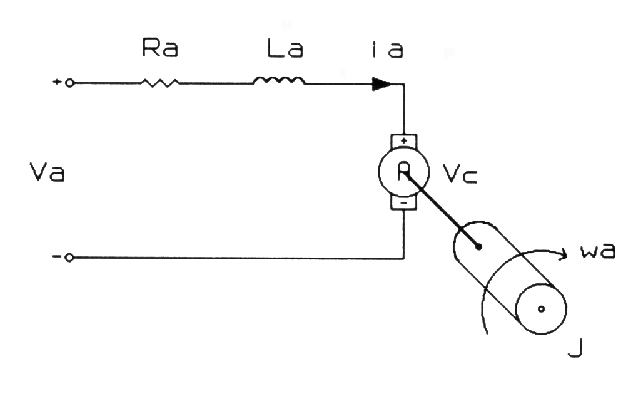
\includegraphics[width=\textwidth]{./img/testrig_dcmotor_model.png}
    \caption{DC motor schematic diagram.}\label{fig:testrig_dcmotor_model}
\end{figure}
Using Kirchhoffs loop rule along with 
\begin{equation} \label{eq:testrig_kphi_v}
    V_C = k_{\phi} \omega
\end{equation}
and 
\begin{equation} \label{eq:testrig_kphi_i}
    T = k_{\phi} \omega
\end{equation}
gives the electric dynamics of the motor,
\begin{equation} \label{eq:testrig_dcmotor}
    \begin{cases} 
        V_A = R_A i_a + L_A \frac{di_a}{dt} + k_{\phi}\omega \\
        J \frac{d\omega} {dt} = k_{\phi} i_a - d\omega - \mu. 
    \end{cases}
\end{equation}
Performing a Laplace transform and rewriting Equation (\ref{eq:testrig_dcmotor})
one gets a second order model for the motor as a transfer function between
voltage and rotational velocity,
\begin{equation} \label{eq:testrig_motor_2ndorder}
    \omega = \frac {k_{\phi}} {(sJ + d) (R_A + sL_A) + k_{\phi}^2} U_A -
    \frac {sL_A + R_A} {(sJ + d) (R_A + sL_A) + k_{\phi}^2} \mu.
\end{equation}
\subsubsection{Model 1}
As a first attempt, the model in Equation (\ref{eq:testrig_motor_2ndorder}) is 
simplified by making the following assumptions:
\begin{enumerate}
    \item Inductance is small enough to be negligible.
    \item Static friction is small enough to be negligible.
\end{enumerate}
With these assumptions
Equation (\ref{eq:testrig_motor_2ndorder}) becomes a first order system,
\begin{equation} \label{eq:testrig_motor_1storder}
    \omega = \frac {k_{\phi}} {sJ + d R_A + k_{\phi}^2} U_A.
\end{equation}
Equation (\ref{eq:testrig_motor_1storder}) can be rearranged to a standard first
order transfer function form, yielding
\begin{equation} \label{eq:testrig_motor_1storder_rewrite}
    \omega = \frac {K} {s T + 1}
\end{equation}
where $K = k(1 + \frac{1} {R d})$ and $T = \frac {J} {\frac{k^2} {R} + d}$.
Using the final value theorem, setting $s = 0$, $K$ can be seen to be the steady
state gain of the system and $T$ is the time constant \cite{reglerteknik2006}.
Seeing how $K$ only depends on one unknown variable, $d$, the model is fit to a
steady state gain first using the viscous friction variable. The inertia $J$ is
then fitted using the time constant of the response and $d$ as a known variable.
The step response with the largest amplitude is used for fitting the data. This
is where the effects of the viscous friction are the largest and it should give
the highest fidelity model available. 

Evaluating the results, it can be seen that the model fits the real system very
well around the set point of 20 V. Figure~\ref{fig:1storder_20} shows the step
response at 20 V. The deviating value in the rise of the is an error induced by
the revolutional velocity capturing algorithm in the microcontroller.
\begin{figure}[H]
    \centering
    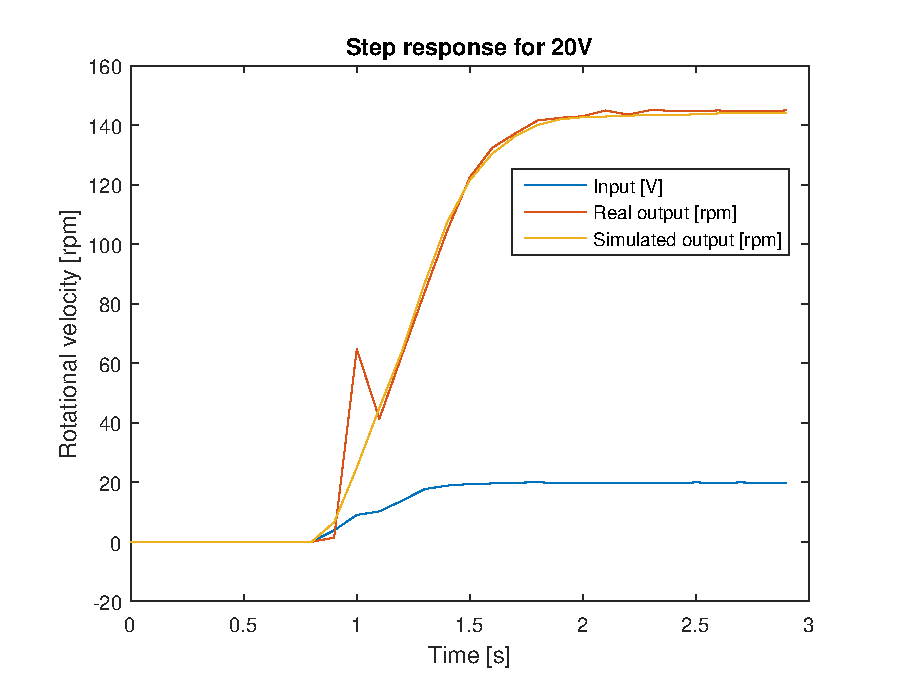
\includegraphics[width=\textwidth]{./img/testrig_20Vstep_no_i_no_fric.eps}
    \caption{Step response for a 1st order model at 20 V.}\label{fig:1storder_20}
\end{figure}
However, the static error increases the further away from the setpoint the tests
are run, see for example Figure~\ref{fig:1storder_5}.
\begin{figure}[H]
    \centering
    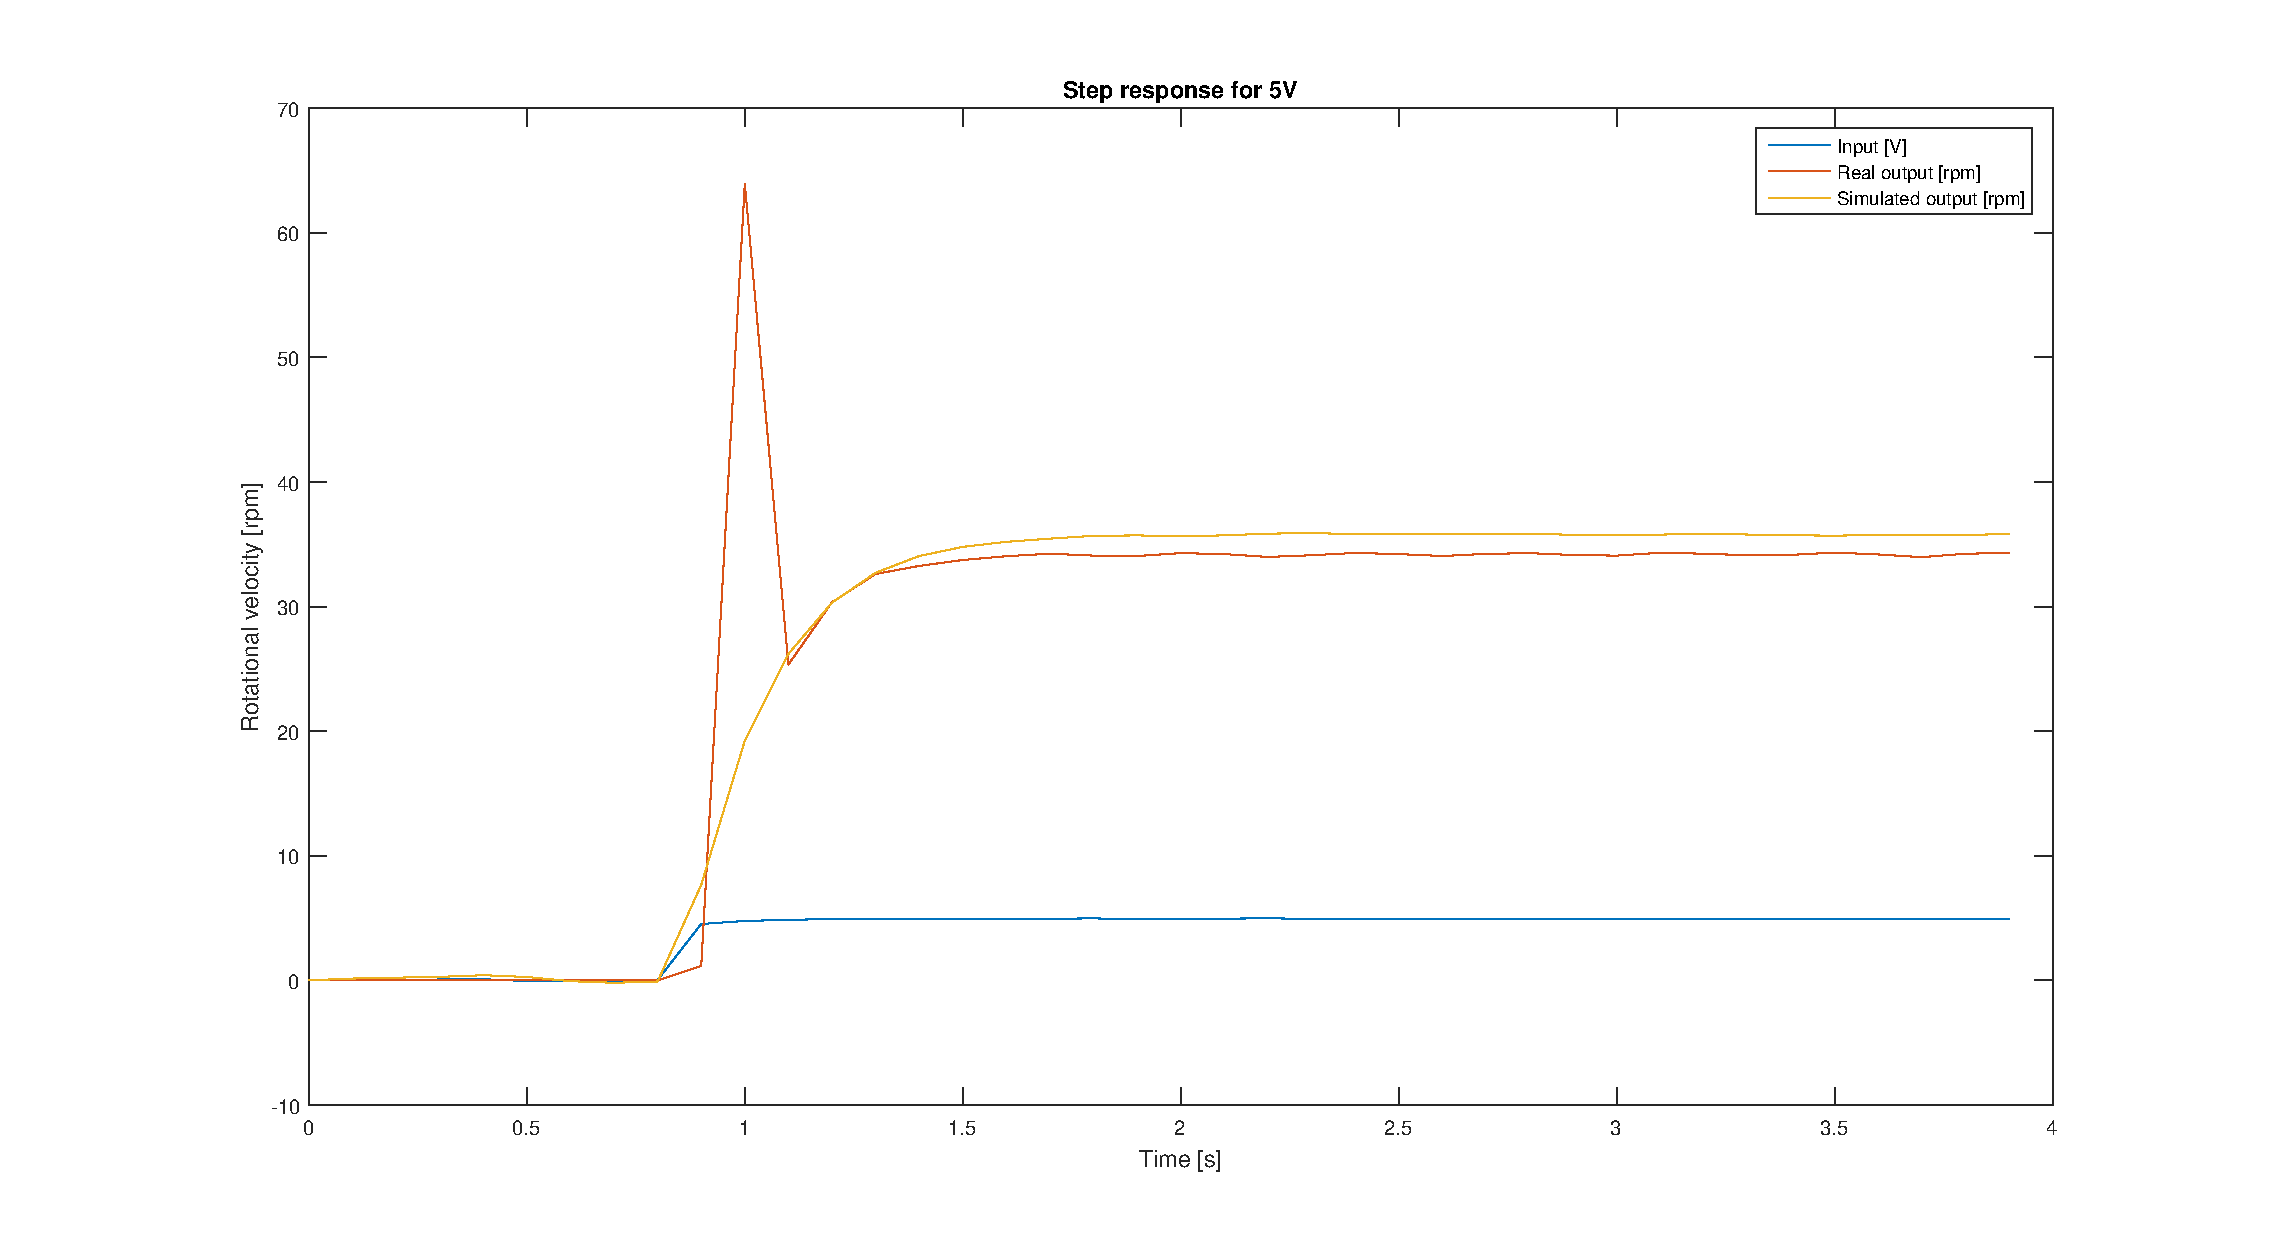
\includegraphics[width=\textwidth]{./img/testrig_5Vstep_no_i_no_fric.eps}
    \caption{Step response for a 1st order model at 5 V. Note the steady state
    error compared to the set point.}\label{fig:1storder_5}
\end{figure}
Also, when validating the model using a sine wave at low amplitude, there is a
significant discrepancy in the model performance compared to the real system at
the turning points. The real system needs to reach a certain voltage before it
can overcome the initial friction whereas the simplified model does not. In 
\begin{figure}[H]
    \centering
    \begin{subfigure}[H]{0.48\textwidth}
    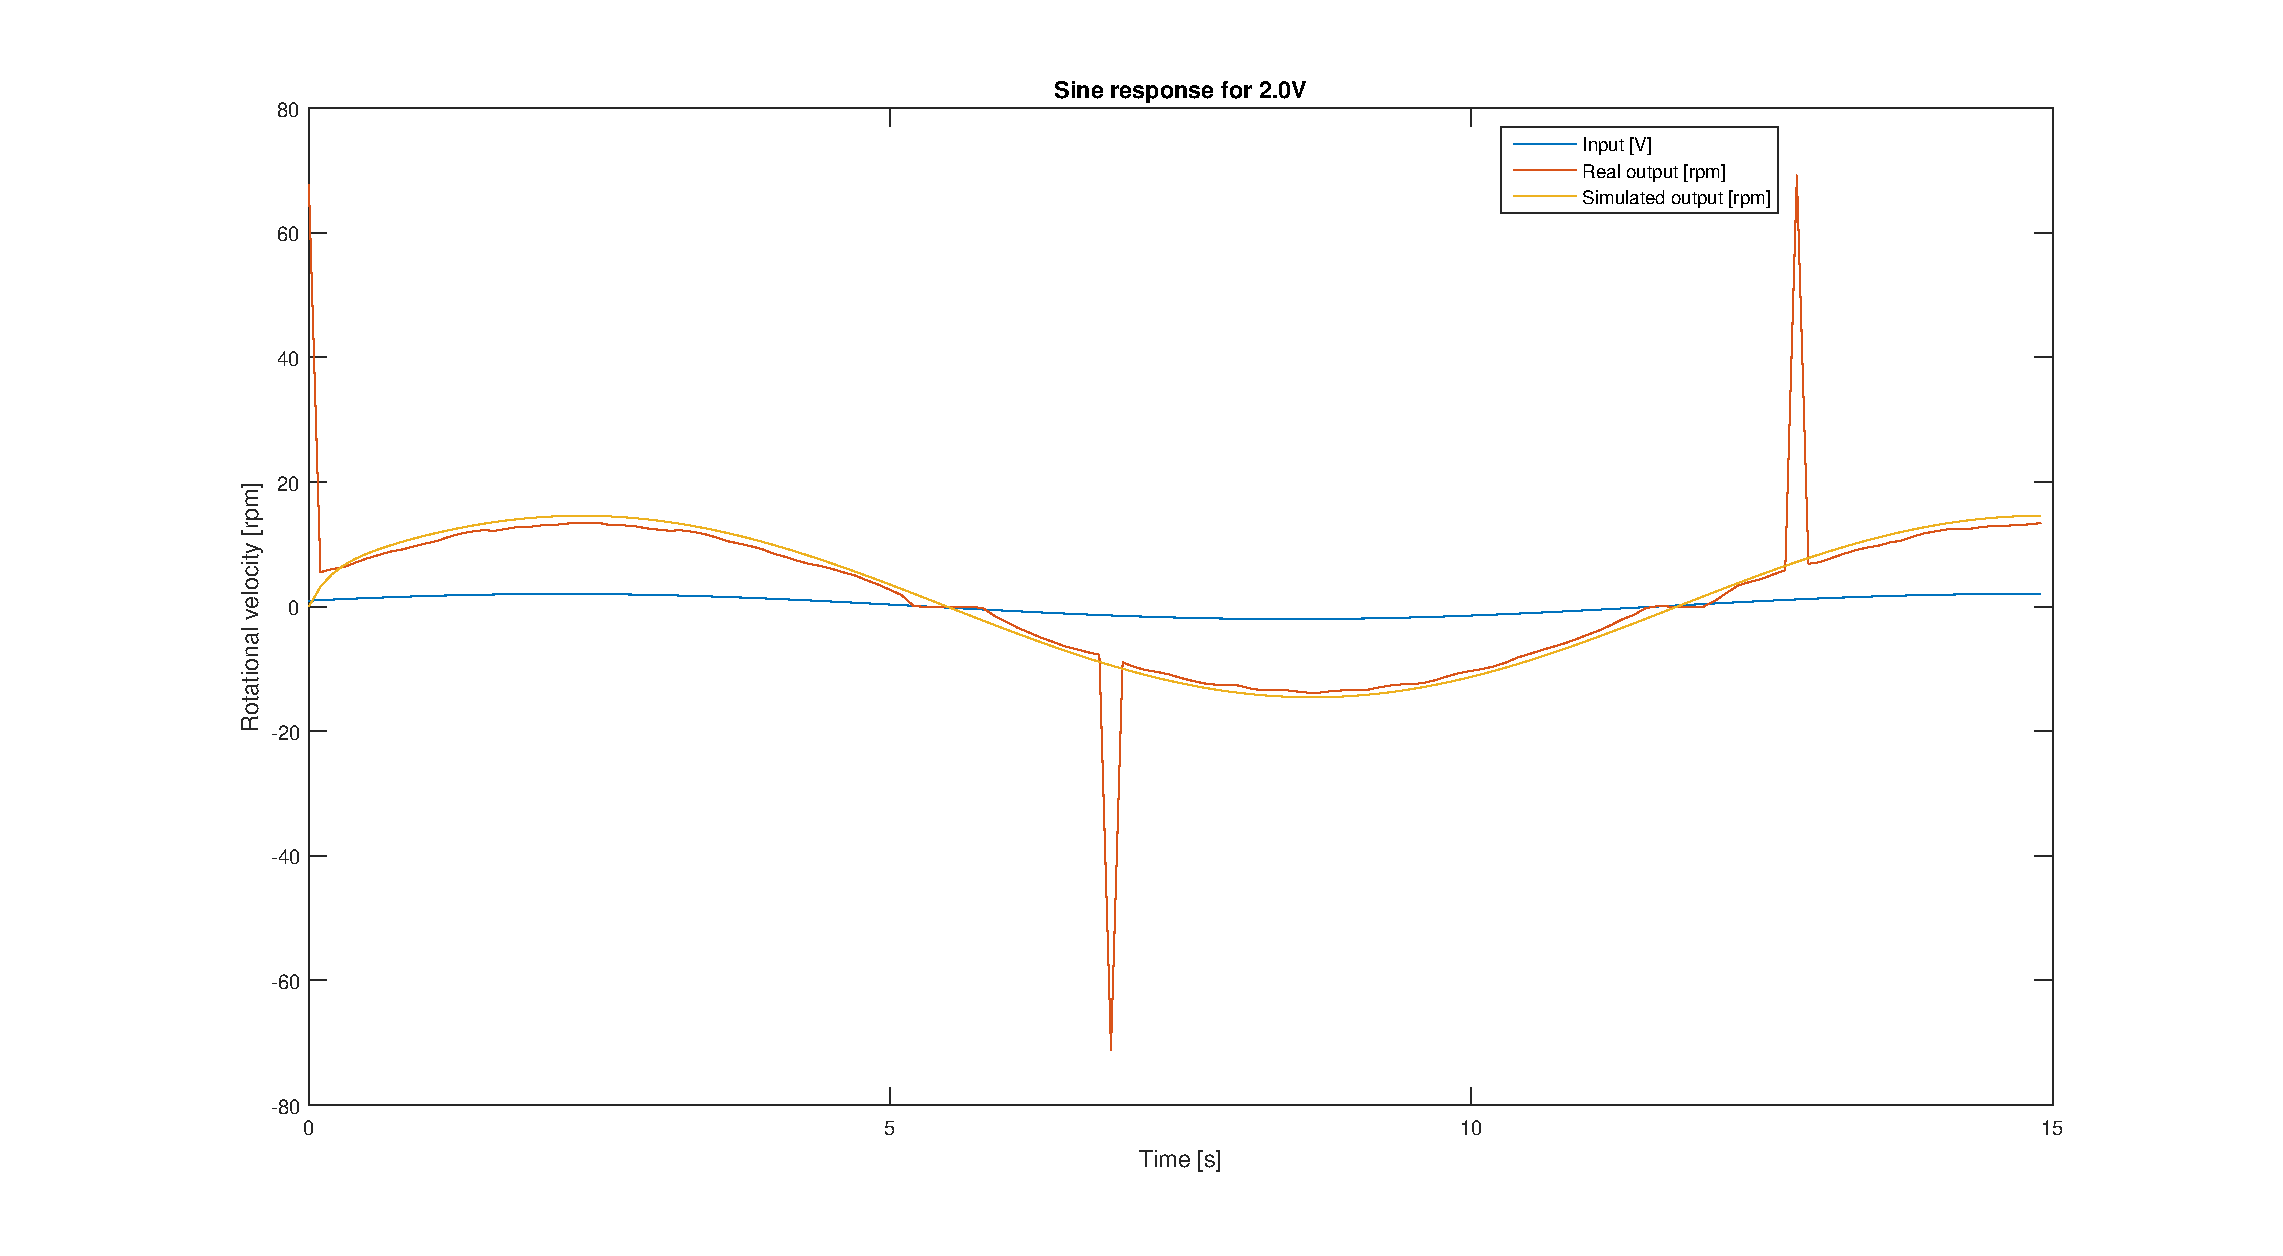
\includegraphics[width=\textwidth]{./img/testrig_2Vsine_no_i_no_fric.eps}
    \caption{Full response.}\label{fig:1storder_sine2}
    \end{subfigure}
    \begin{subfigure}[H]{0.48\textwidth}
    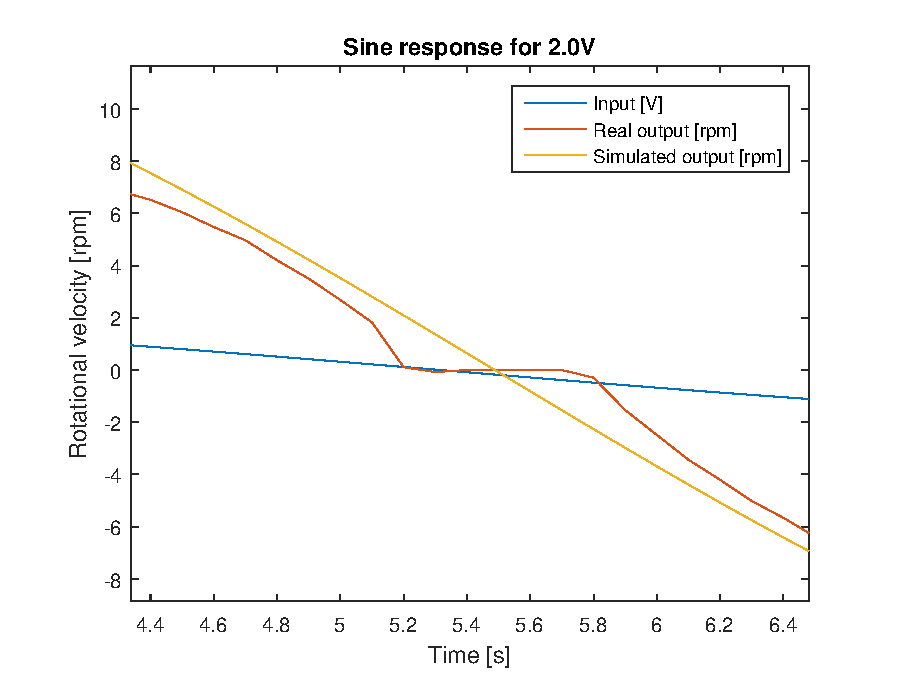
\includegraphics[width=\textwidth]{./img/testrig_2Vsine_no_i_no_fric_zoom.eps}
    \caption{Magnification on turning point.}
    \end{subfigure}
    \caption{Sine response for first order model with no inductance or static
    friction.}\label{fig:1storder_sine2z}
\end{figure}
The full set of step and sine responses for this model are given in
Appendix~\ref{app:identification}.

\subsubsection{Model 2}
The previous model showed good correspondence for the time constant but had a
steady state error when not at the set point. It also did not catch the dynamics
at the turning of the rig. There is a missing dynamic that is not captured with
the simple model. The fact that there is a threshold needed for the testrig to
start turning hints that a static friction is present in the system and that it
is significant enough to directly affect the dynamics in a noticeable way.
Therefore, the model fitting is reiterated with a model that takes the static
friction into account and only makes the assumption that the effect of the motor
inductance is negligible. The new model achieved is then
\begin{equation} \label{eq:model2}
    \omega = \frac {k_{\phi}} {sJ + d R_A + k_{\phi}^2} U_A -
    \frac {R_A} {sJ + d R_A + k_{\phi}^2} \mu.
\end{equation}
A static friction is a disturbance torque that at its simplest has a constant
amplitude and changes with the direction of velocity. This representation is not
suitable for numerical solving because of the discontinuity that occurs when the
system turns. To counter this, a stick-slip region is added around the origin,
i.e. the turning point. Within this stick-slip region, the friction force is
equal to the internally applied torque from the motor until the static friction
maximum value is reached. After that, the friction torque is constant. This
friction model is called the Karnop friction model, see Figure~\ref{fig:karnop}.
\begin{figure}[H]
    \centering
    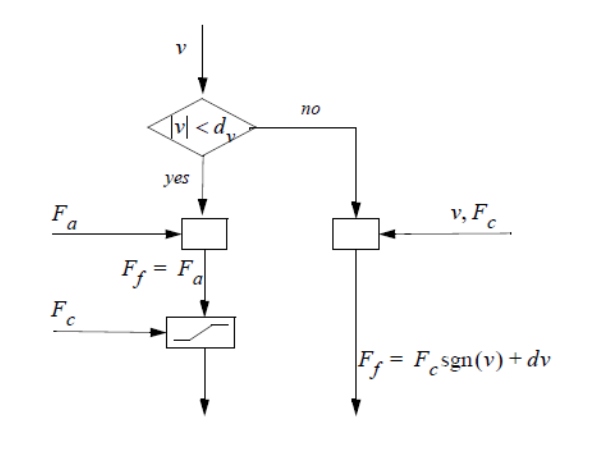
\includegraphics[width=\textwidth]{./img/testrig_karnoplogic.png}
    \caption{Schematic of Karnop logic. $v$ is velocity, $F_C$ is Karnop
    friction, $F_a$ is applied force, $d_v$ is velocity threshold and $F_f$ is
friction force. Image from lecture series in MF2007 Dynamics and motion control
at KTH, courtesy of Dr Lei Feng.}
    \label{fig:karnop}
\end{figure}
Karnop allows numerical solvers to be used on the model but it also introduces 2 new
parameters to fit. These are the static Coulomb friction $F_C$ and the velocity
threshold $d_v$.

To successfully fit the parameters of the model, a systematic approach based on
the physical effects of the parameters is used. The viscous friction and inertia 
is firstly estimated at the largest input step. At this point, viscous friction
should be dominant over the static friction, allowing a good estimate of these
parameters with as little disturbance as possible. After a good model is found,
the two static friction parameters are fitted by trial and error. Lastly, the
model is fitted to the largest step again, fine tuning the inertia and viscous
friction parameters.

The model now follows the real response of the system at all three step sizes,
with a very small steady state error. Step response for the edge cases are shown
in Figure~\ref{fig:20vkarnop} and~\ref{fig:5vkarnop}.
\begin{figure}[H]
    \centering
    \begin{subfigure}[H]{0.48\textwidth}
    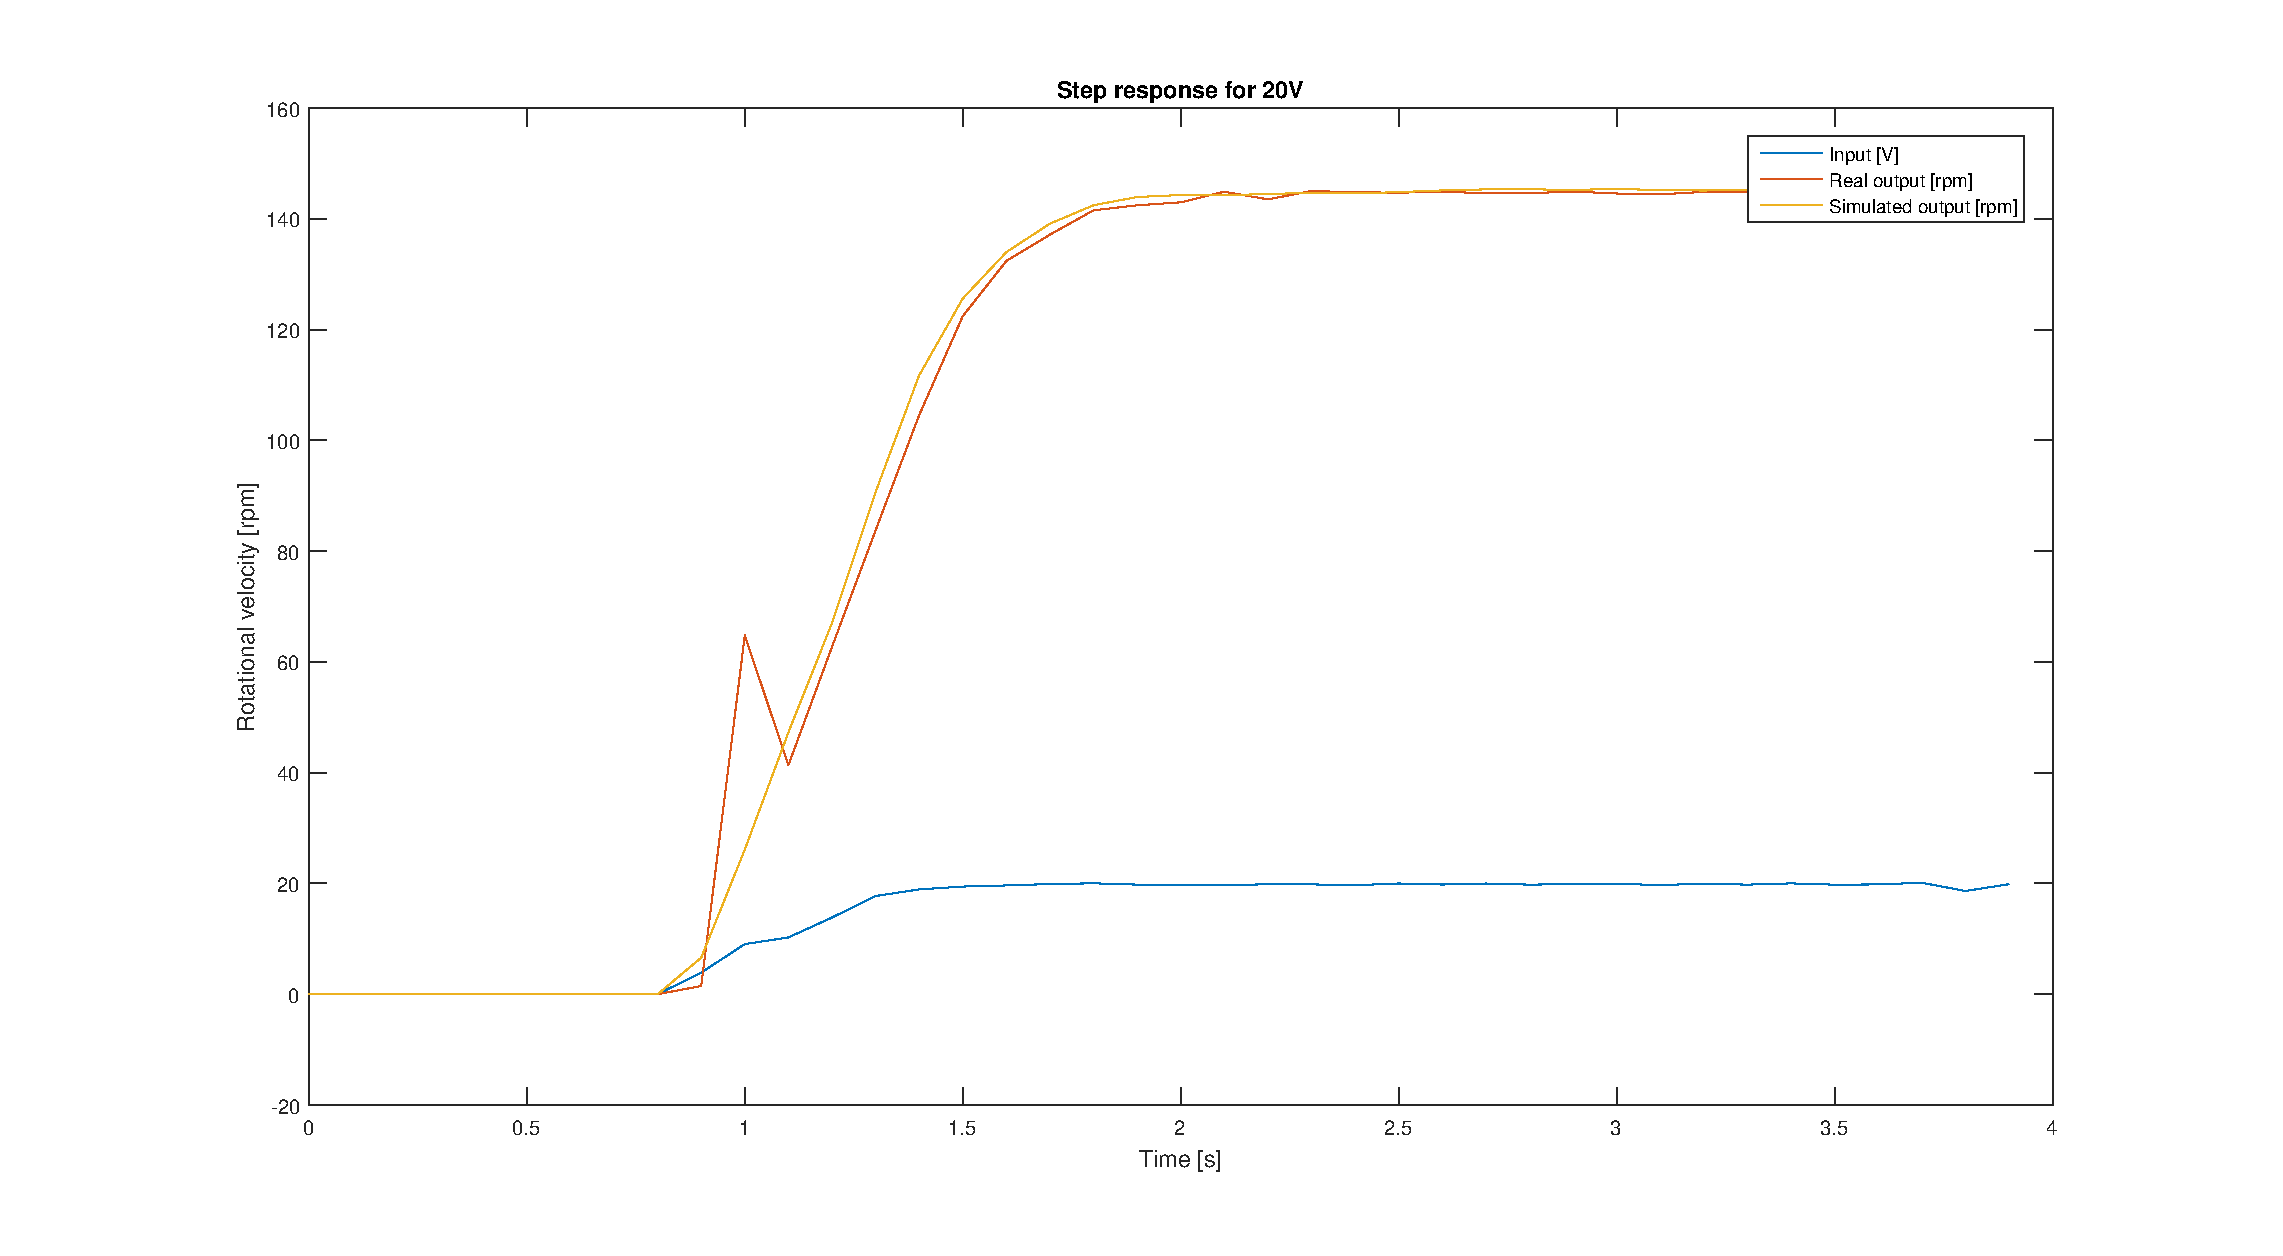
\includegraphics[width=\textwidth]{./img/testrig_20Vstep_no_i_fric.eps}
    \caption{20 V step input.}\label{fig:20vkarnop}
    \end{subfigure}
    \begin{subfigure}[H]{0.48\textwidth}
    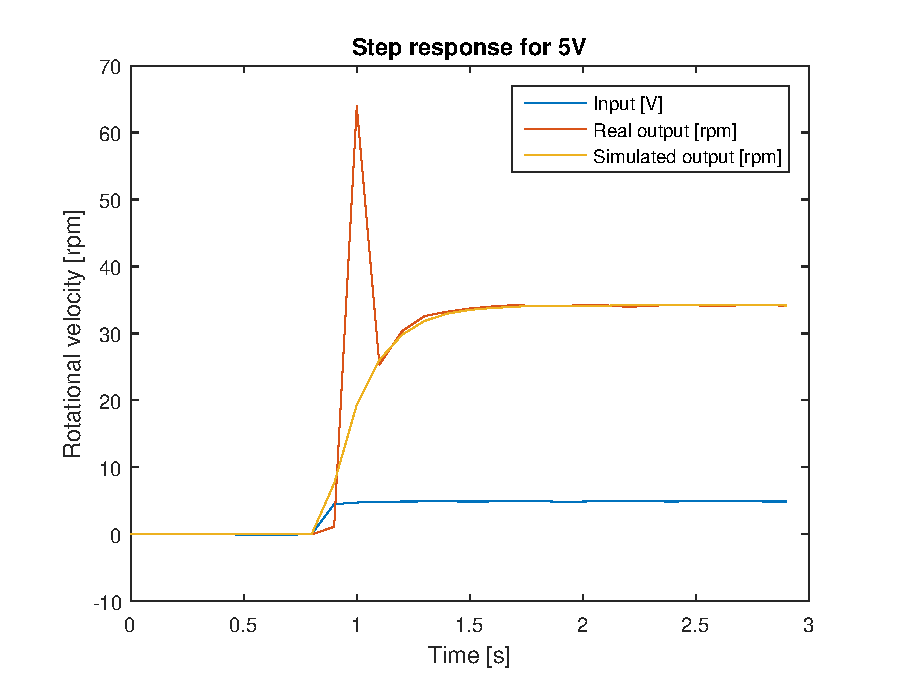
\includegraphics[width=\textwidth]{./img/testrig_5Vstep_no_i_fric.eps}
    \caption{5 V step input.}\label{fig:5vkarnop}
    \end{subfigure}
    \caption{Step responses for the edge case of the first order system with
    Karnop friction.}
\end{figure}
The steady state error has a maximum error of 1.5\% over all three input step
sizes and the rise time has a maximum deviation of 4.1\%. There is
an area at low speeds in which the model and the real system do not correlate
well but the real system and the model converge at the end of the step inputs. 

In the validation step, the model follows the behaviour of the real system well.
In Figure~\ref{fig:1storder_f_sine2} and~\ref{fig:1storder_f_sine2z}, it can be
seen that the model follows the real system well in the turning point. However,
there is a static following error but this was not part of the requirements. The
model is therefore accepted as suitable. The full set of step and sine responses
are given in Appendix~\ref{app:identification}
\begin{figure}[H]
    \centering
    \begin{subfigure}[H]{0.48\textwidth}
    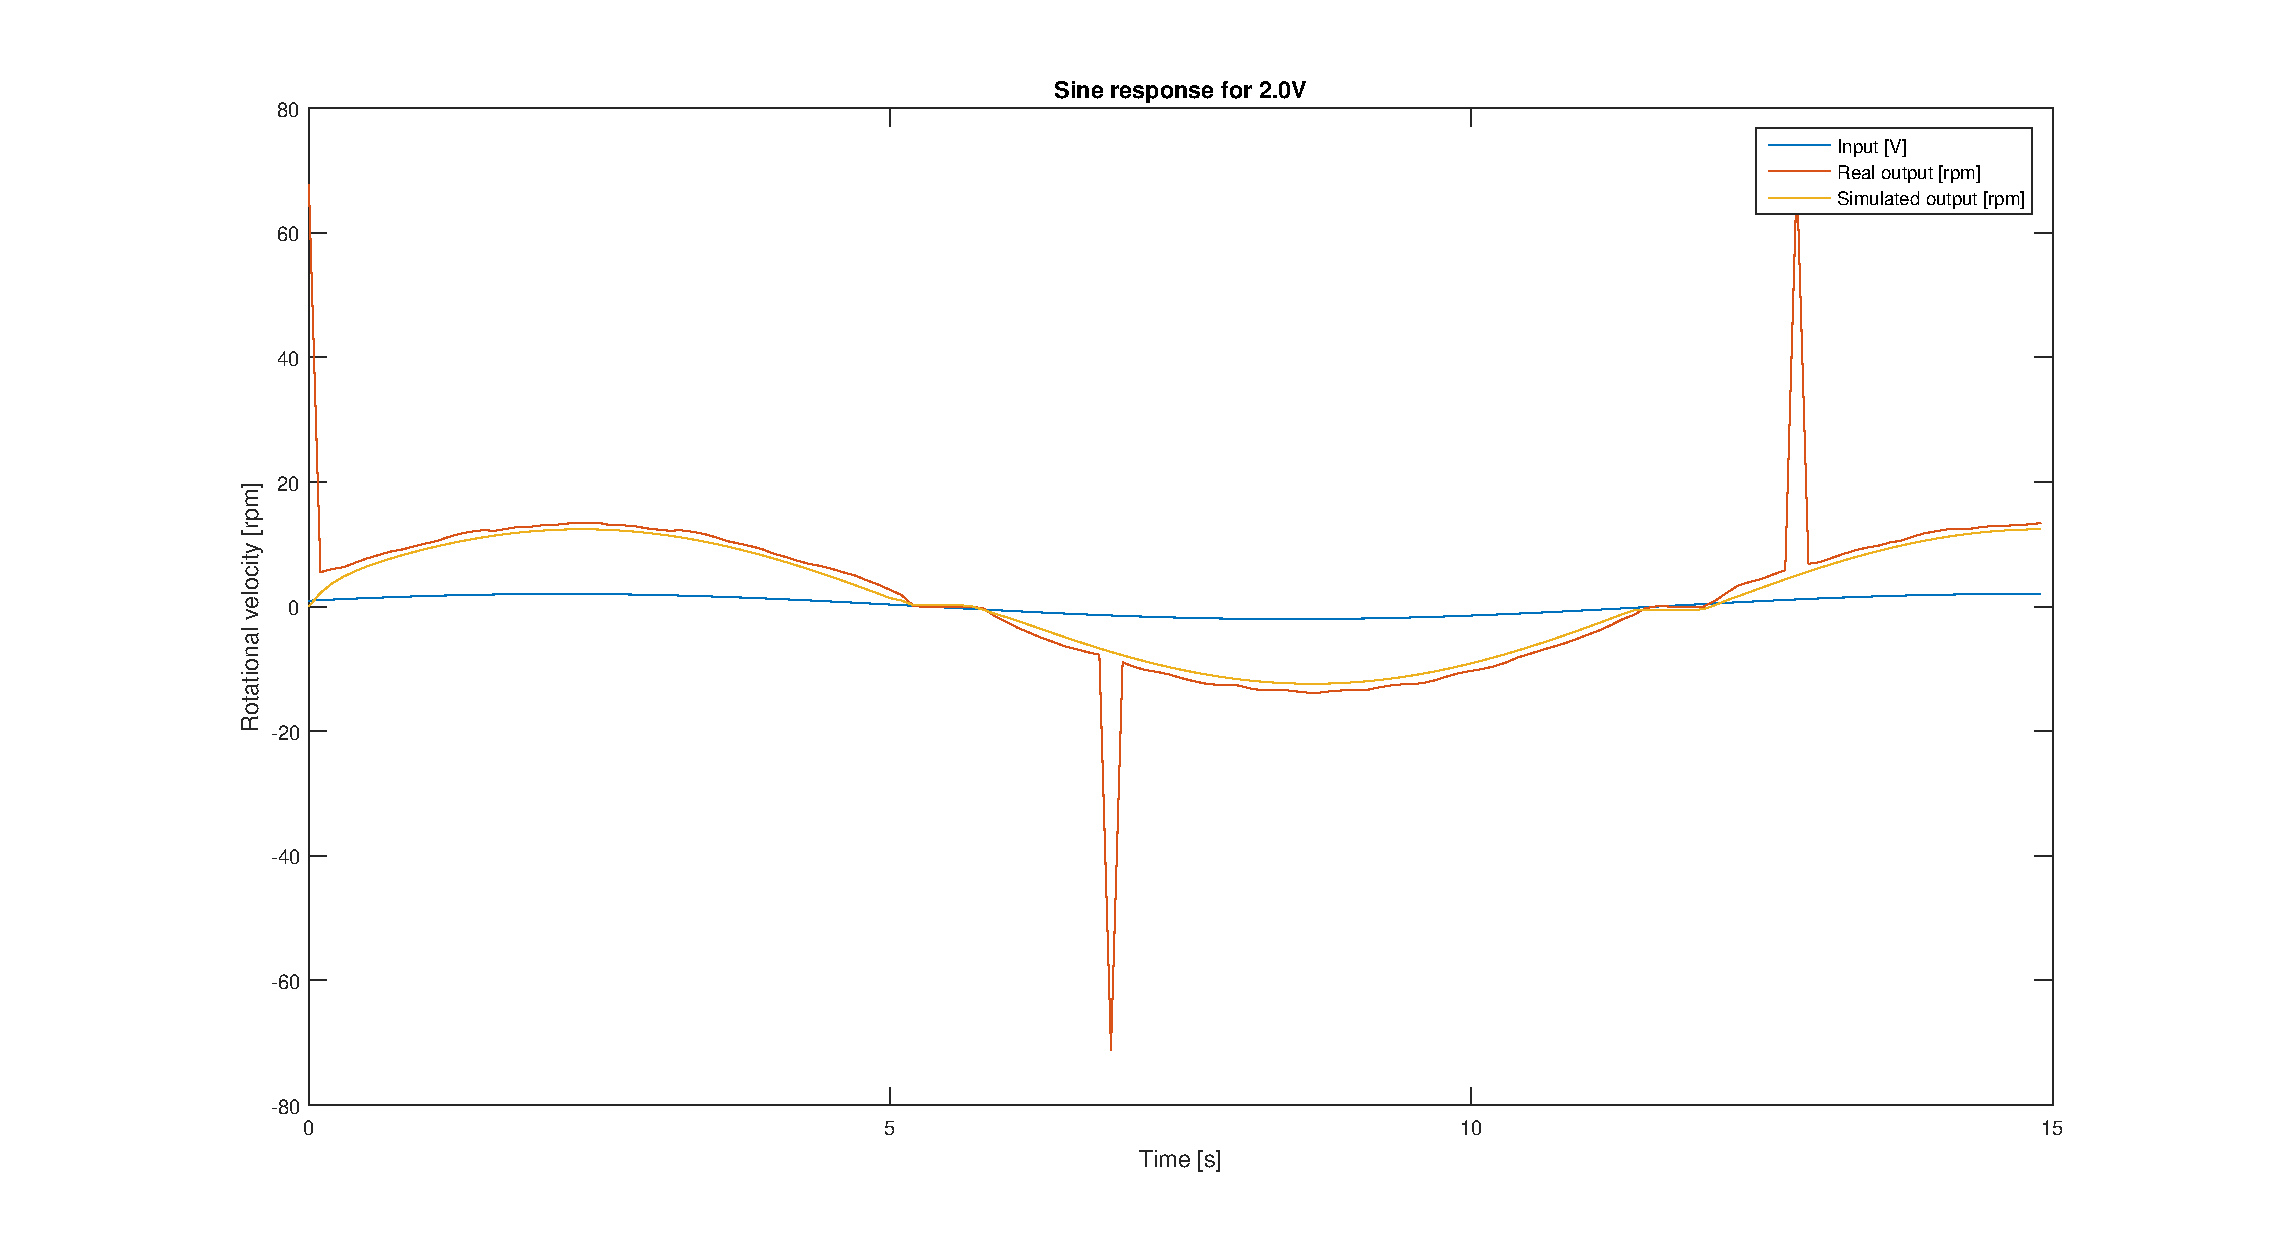
\includegraphics[width=\textwidth]{./img/testrig_2Vsine_no_i_fric.eps}
    \caption{Full response.}\label{fig:1storder_f_sine2}
    \end{subfigure}
    \begin{subfigure}[H]{0.48\textwidth}
    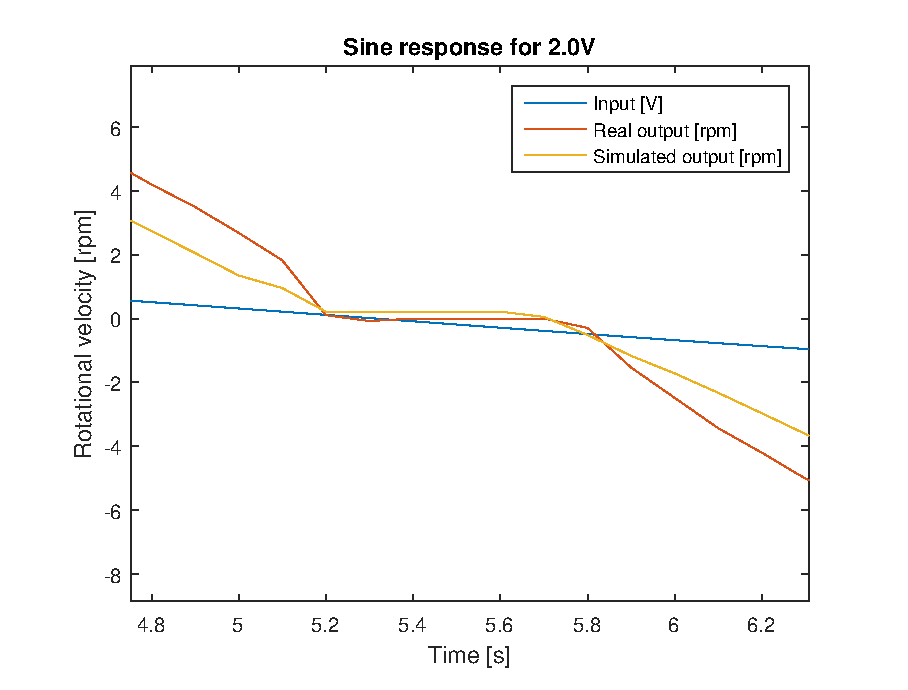
\includegraphics[width=\textwidth]{./img/testrig_2Vsine_no_i_fric_zoom.eps}
    \caption{Magnification on turning point.}\label{fig:1storder_f_sine2z}
    \end{subfigure}
    \caption{Sine response for first order model with static Karnop friction and 
    no inductance.}
\end{figure}

\subsection{Result analysis}
In summary, a first order model in which the effects of the inductance are
ignored is used. Friction is modeled using the Karnop model with a stick-slip
area at low rotational velocities and a viscous friction outside the stick-slip
zone. The inertia of the model $J$ is $0.0135 \si{\kilogram\second^{2}}$ and the
viscous friction $d$ is $0.078 \si{\newton\meter\per\radian\second}$. The
stick-slip threshold $d_v$ is $0.01 \si{\radian\per\second}$ and the static
Coulomb friction $F_C$ is $0.02 \si{\newton\meter}$. The value of the inertia is
considered to be feasible. There are no exact measurements available for the
internal diameter of the roller but an estimation made in Solid Edge gives a
moment of inertia of $0.022 \si{kilogram\meter^{2}}$. Being a rough estimation,
it gives an indication on that the inertia estimation is correct. The estimated
value of $d$ is rather high, considering that there will be roughly 1 Nm of
viscous friction torque for every 12 rad/s of motor speed. This can be expected
of the system. Misalignments and the chain-drive most likely adds a significant
amount of viscous friction. Static torque is comparatively small compared to
other losses in the system which might be because of the magnitude of the
viscous friction. The static friction does however have an important effect on
the system and cannot be ignored. The model fulfils the requirements and is
considered to be good enough to use in the final system.
